\documentclass[11pt]{article}
\usepackage[utf8]{inputenc}
\usepackage[a4paper, total={6in,8in}, portrait, margin=1in]{geometry}
\usepackage{amssymb}

%Add any packages you need here
\usepackage{graphicx}
\usepackage{amsmath}
\usepackage{amsfonts}
\usepackage{float}
\usepackage{natbib}
\usepackage{algpseudocode}
\usepackage{listings}
\usepackage[misc]{ifsym}
\usepackage{indentfirst} 
\usepackage{amsthm}
\usepackage{appendix}
\usepackage{dirtree}
\usepackage{xcolor}

%Any functions you wanna define, pop 'em here
\newtheorem{theorem}{Theorem}[section]
\newtheorem{remark}[theorem]{Remark}
\newtheorem{definition}[theorem]{Definition}
\newtheorem{example}[theorem]{Example}
\newtheorem{lemma}[theorem]{Lemma}

\definecolor{codegreen}{rgb}{0,0.6,0}
\definecolor{codegray}{rgb}{0.5,0.5,0.5}
\definecolor{codepurple}{rgb}{0.58,0,0.82}
\definecolor{backcolour}{rgb}{0.95,0.95,0.92}

\lstdefinestyle{mystyle}{
    backgroundcolor=\color{backcolour},   
    commentstyle=\color{codegreen},
    keywordstyle=\color{magenta},
    numberstyle=\tiny\color{codegray},
    stringstyle=\color{codepurple},
    basicstyle=\ttfamily\footnotesize,
    breakatwhitespace=false,         
    breaklines=true,                 
    captionpos=b,                    
    keepspaces=true,                 
    numbers=left,                    
    numbersep=5pt,                  
    showspaces=false,                
    showstringspaces=false,
    showtabs=false,                  
    tabsize=2
}

\lstset{style=mystyle}



\title{Barrier Options Pricing Under Local Volatility - Developer Documentation}
\author{Matthew Knowles}
\date{January 202}

\begin{document}

\maketitle

\section{Project Structure}

There are 5 .m files included in this project. The file ``main.m'' works only as a wrapper for the other files that price options using different methods. 
This can be seen in the following directory tree. 

\begin{figure}[h]
    \caption{Project Structure}
    \dirtree{%
    .1 /.
    .2 Documentation.
        .3 devdoc.pdf.
        .3 userinstructions.pdf.
    .2 main.m.
    .2 implicit.m.
    .2 explicit.m.
    .2 crank.m.
    .2 monte\_carlo.m.
    }
\end{figure}

\section{Functions}

The files ``implicit.m'', ``explicit.m'' and ``crank.m'' contain a function of the same name, taking the imputs: $S0, K, B, r, q, T, N, M$ and outputs a price 
calcualted by the respective scheme that the function implements. The ``implicit.m'' and ``crank.m'' functions contain a function ``tridiag'', written by Dr. Francesco 
Cosentino for solving the matrix equation $Ax=b$ for a tridiagonal matrix $A$. The file ``monte\_carlo.m'' takes slightly different inputs. This is because 
instead of a grid requiring the parameter $N$, we require a number of simmulations $Nmc \in \mathbb{N}$. ``monte\_carlo.m'' therefore takes the parameters
$S0, K, B, r, q, T, Nmc, M$. The parameter $M$ is used in calculating payoffs. Simply running the ``main.m'' script will print 4 prices, one for each scheme.

\section{Further Details}
Across the three FDM methods, the first few parts of each script are virtually unchanged. Namely, we create a grid of points between $S_{min}$ and $S_{max}$
and one between $0$ and $T$. We then create the first vector, $V$ of initial option prices, using a for-loop to set $V_j= max(S_j-k,0)$ if $S_j < B$, or 0 otherwise. 
Then the local volatility is calculated at each point on the grid. By extension, we then calculate $\alpha$ and $\beta$ at each gridpoint. This is all done 
using nested for-loops due to ease of reading. \\

Each script then diverges into their own algorithms. This usually involves calculating the matrices containing the $d_{j,k} \ u_{j,k}$ and $l_{j,k}$ values. 
The actual solving of the Black-Scholes equation is done in a for-loop incramenting from a step $k$ to $k+1$, updating $V = Vnew$ after each new calculation. \\

The Monte-Carlo method takes a different method, but calculating random stock movements, by making use of the MATLAB function ``randn'' to generate sample 
values from the $N(0,1)$ distribution. We use antithetic-sampling to reduce variance in the calculation. However due to the computationally intensive nature of 
antithetic sampling, we calculate the determinsitc and drift terms in the equation only once, which cuts runtime in half. The monte-carlo method script could be 
extended in future work by using control variables. This would of course increase computation time, but it would reduce the variance by a factor of $\beta^2$, where 
$\beta$ is the corrolation coefficient between $X_i$ and $Y_i$.

\section{Testing}

\subsection{Antithetic Sampling for Variance Reduction}
Antithetic Sampling is used to reduce the variance in a model by introducing negatively corrolated samples. 

\begin{figure}[h]
    \centering
    \begin{minipage}{0.4\textwidth}
        \centering
        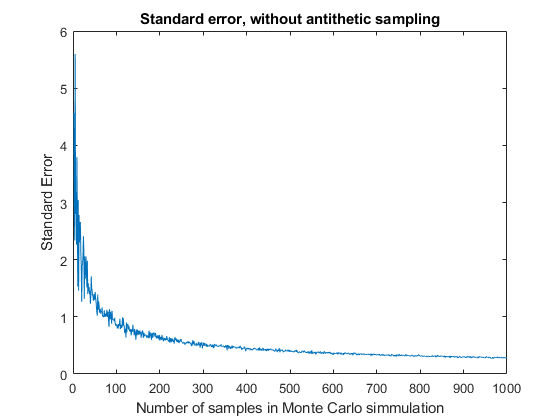
\includegraphics[width=1.1\textwidth]{StandardError.png}
        \caption{Standard Error without Antithetic Sampling}
    \end{minipage}
    \begin{minipage}{0.4\textwidth}
        \centering
        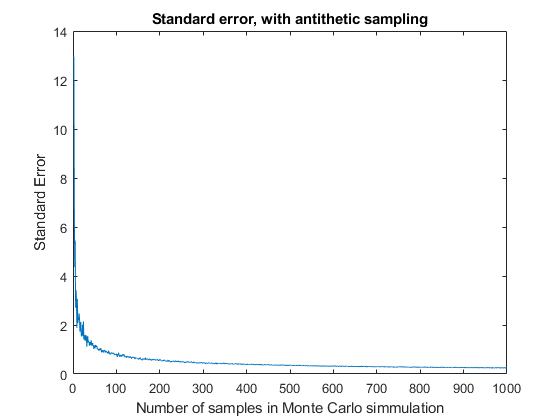
\includegraphics[width=1.1\textwidth]{StandardErrorAT.png}
        \caption{Standard Error with Antithetic Sampling}
    \end{minipage}
\end{figure}

We can see from the standard error graphs that both errors tend to 0 as the number of simmulations increases, 
although we can see that the line in the antithetic sampling figure is much thinner, due to the overall reduction 
in variance. \\

\subsection{Variable Grid Sizing in FDM Schemes}
Starting with a $N=500, M=1000$ grid, we increased each one by 10 each time, and used the three FDM schemes to price the same barrier option.
The curves showing how price varies with grid size is showing in Figure~\ref{gridsize}. What is interesting is how the Implicit scheme 
takes longer to approach the price than the other two schemes, which consistently stay around 10. 

\begin{figure}[h]
    \centering
    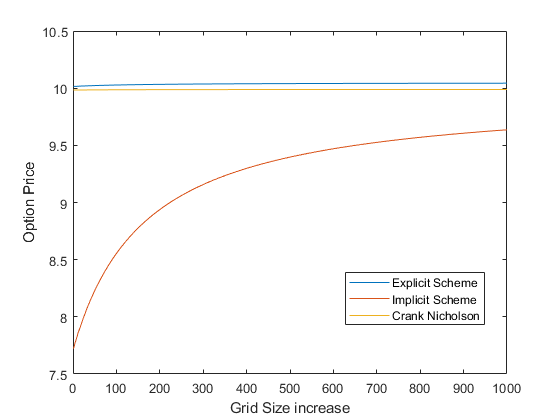
\includegraphics[width=0.5\textwidth]{gridtest.png}
    \caption{Price change with Variable Grid Size}
    \label{gridsize}
\end{figure}

Since we don't have an analytic to the PDE, we compare our prices with the monte-carlo simmulation. This consistently floated around 10 for 
varying values of $Nmc$. The Implicit scheme appears to converge to the true value, although it is computationally expensive to find a grid large 
enough for which this is the case. 


\subsection{Performance}
Including antithetic sampling in the Monte-Carlo simmulation greatly increases. The below table shows how the 
time to run changes with increasing number of simmulations both using and not using antithetic sampling.


\begin{table}[h]
\centering
\begin{tabular}{c c c c c}
    Nmc &  \vline & Non-Antithetic Time (s)& Antithetic Time (s) & Improved Antithetic Time (s) \\
    \hline
    100 &  \vline & 0.0454 & 0.0691 & 0.0397 \\
    1000 & \vline & 0.3588 & 0.7000 & 0.3777 \\
    10000 & \vline & 3.6219 & 7.002 & 3.9213 \\
    100000 & \vline & 35.7083 & 71.5724 & 39.3678 
\end{tabular}
\caption{Table showing performance times for different versions of the Monte-Carlo method}
\label{MCTable}
\end{table}

We can see that although both increase exponentially, the version using antithetic sampling ends up roughly 
doubling the time taken by not using it. This is because we are calculating double the amount of samples, just with 
opposite coefficient on the drift term. So in order to increase performance, it was decided that instead of 
calculating $(r-\delta-\frac{\sigma^2}{2})(t_{i+1}-t_i)$ and $\sigma\sqrt{t_{i+1}-t_i}$ twice, we can calculate them at 
the start of the for-loop and call that value when it is needed. It can be seen in the final column of Table~\ref{MCTable}
that doing this cuts the time down by again around a half, so we get the reduced variance and increased performance.

\end{document}